\documentclass[11pt]{article}

\linespread{1.1}

\usepackage{polski}
\usepackage[utf8]{inputenc}

\usepackage{graphicx}
\usepackage[unicode]{hyperref}
\usepackage{fancyhdr}
\usepackage{geometry}
\geometry{a4paper, left = 2.5cm, right = 2.5cm, top = 2.5cm, bottom = 2.5cm}
\usepackage{indentfirst}
\usepackage[dvipsnames, table]{xcolor}
\usepackage{amsmath}
	\DeclareMathOperator{\matA}{\boldsymbol{A}}
	\DeclareMathOperator{\matB}{\boldsymbol{B}}
	\DeclareMathOperator{\matR}{\boldsymbol{R}}
	\DeclareMathOperator{\matQ}{\boldsymbol{Q}}
	\DeclareMathOperator{\matF}{\boldsymbol{F}}
	\DeclareMathOperator{\matK}{\boldsymbol{K}}
	\DeclareMathOperator{\matx}{\boldsymbol{x}}
	\DeclareMathOperator{\matu}{\boldsymbol{u}}
	\DeclareMathOperator{\matI}{\boldsymbol{I}}
	
\usepackage{subfig}
\usepackage{multirow}
\usepackage{tikz}
	\usetikzlibrary{shapes, arrows, positioning}
\usepackage{tabularx}
\usepackage{booktabs}
\usepackage{siunitx}
\usepackage{pgfplots}
\usepackage{listings}
\usepackage{colortbl}
\usepackage[shortlabels]{enumitem}
\usepackage[title]{appendix}

\usepackage{ifthen}
	\newcounter{num}
	\setcounter{num}{0}

% \captionsetup[subfigure]{labelformat = empty}

\definecolor{codegray}{rgb}{0.5, 0.5, 0.5}
\definecolor{codepurple}{rgb}{0.58, 0, 0.82}
\definecolor{backcolour}{rgb}{0.95, 0.95, 0.92}

\definecolor{tableGray}{rgb}{0.9, 0.9, 0.9}

\renewcommand{\arraystretch}{1.2}

\lstdefinestyle{mystyle}{%
	backgroundcolor = \color{backcolour},
% 	basicstyle = \ttfamily \small,
 	basicstyle = \ttfamily \footnotesize,
	commentstyle = \color{red!90},
	numberstyle = \tiny \color{codegray},
	stringstyle = \color{codepurple},
	breakatwhitespace = false,
	breaklines = true,
	captionpos = b,
	keepspaces = true,
	showspaces = false,
	showstringspaces = false,
	showtabs = false,
	tabsize = 4,
	numbers = left,
	numberstyle = \tiny \color{black},
	morecomment = [l]{\%},
	frame = single
}

\lstset{%
	style = mystyle,%
	literate = %
		{ą}{{\k{a}}}1
		{Ą}{{\k{A}}}1
		{ć}{{\'c}}1
		{Ć}{{\'{C}}}1
		{ę}{{\k{e}}}1
		{Ę}{{\k{E}}}1
		{ł}{{\l{}}}1
		{Ł}{{\L{}}}1
		{ń}{{\'n}}1
		{Ń}{{\'N}}1
		{ó}{{\'o}}1
		{Ó}{{\'O}}1
		{ś}{{\'s}}1
		{Ś}{{\'S}}1
		{ż}{{\.z}}1
		{Ż}{{\.Z}}1
		{ź}{{\'z}}1
		{Ź}{{\'Z}}1
}

\pgfplotsset{compat = newest}
\usepgfplotslibrary{units}

\sisetup{
	round-mode = places,
	round-precision = 2
}

\linespread{1.1}

\graphicspath{{./img/}}

\pagestyle{fancy}
\fancyhf{}
\lhead{MO -- Projekt}
\rhead{Kaźmieruk, Skibiński}
\cfoot{\thepage}


\setcounter{num}{0}


%%%
%%%		DOKUMENT
%%%

\begin{document}

\ifthenelse{\equal{\value{num}}{0}}{
\begin{titlepage}
	\begin{center}
		\textbf{\LARGE Metody Optymalizacji\\%
		\vspace{1cm}%
		Projekt -- Zbrojenie%
		}
		
		\vspace{0.75cm}
		
		\vspace{1.0cm}
		
		{\large \textbf{AiR S2-I/Rob}}
		
		\vspace{0.2cm}
		
		{\large \textbf{Sekcja nr 1}}%
		
		\vspace{0.5cm}
		
		{\large
		Paweł Kaźmieruk\\
		Maksymilian Skibiński%
		}
		
		\vspace{0.2cm}

		\vspace{2.0cm}
		
		\vfill
		
		\begin{figure}[h]
			\centering
			\includegraphics[trim = 0 20mm 0 0, clip, width = 0.2\linewidth]{C:/good_folder/nauka/inne/polsl_logo}
		\end{figure}
		
		
		\vspace{0.5cm}
		
		Wydział Automatyki, Elektroniki i Informatyki\\
		Politechnika Śląska\\
		11 czerwca 2021 r.%
	\end{center}
\end{titlepage}
\setcounter{page}{2}
}{}

\ifthenelse{\equal{\value{num}}{0} \OR \equal{\value{num}}{1}}{
\section{Wstęp}

Celem tych ,,trwających'' od kilku tygodni zajęć laboratoryjnych, było przetłumaczenie zadania z treścią na problem optymalizacji. Chodzi nam zatem o to, by to co zostało zapisane słowami, zapisać za pomocą języka matematyki, najlepiej w taki sposób, by przypominało to problemy z którymi spotykaliśmy w ramach wykładów/laboratoriów z Metod Optymalizacji.

Nasza sekcja otrzymała zadanie dotyczące zbrojenia protokątnego fundamentu płytowego. W problemie chodzi o to, że należy zakupić całkiem sporą ilość drutu zbrojeniowego, a chcemy zapłacić jak najmniej.

\newpage
}{}

\ifthenelse{\equal{\value{num}}{0} \OR \equal{\value{num}}{2}}{
\section{Drut zbrojeniowy}

\subsection{Przykład}
Zacznijmy od przeanalizowania tego jakie możliwości daje nam sklep, abstrahując od reszty całego zadania:
\begin{itemize}[--]
\item pręty są sprzedawane w rozmiarze $e$ [m],
\item możemy je ciąć dowolną ilość razy na mniejsze części -- tzw. ,,podpręty''.
\end{itemize}

Graficznie wygląda to tak:
\begin{figure}[h!]
	\centering
	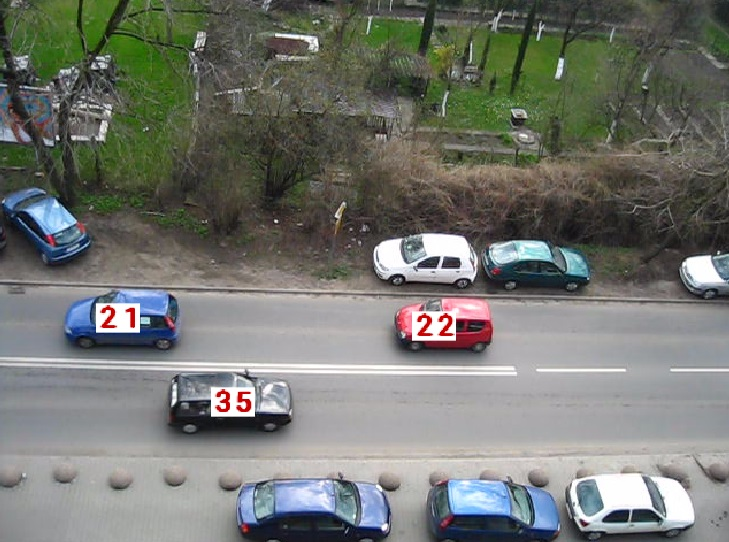
\includegraphics[width = 0.5 \linewidth]{img1}
	\caption{Przykładowe zakupy w sklepie}
\end{figure}

Na rysunku powyżej sytuacja wygląda w następujący sposób:
\begin{itemize}[--]
\item zakupionych zostało 5 prętów,
\item wszystkie mają tę samą długość $e$ m,
\item niektóre z nich zostały zakupione w całości, a pozostałe zostały pocięte:
\begin{itemize}[--]
\item pręt nr 1 jest w całości,
\item pręt nr 2 został zakupiony w dwóch, właściwie równych, częściach,
\item pręt nr 3 został zakupiony w trzech częściach,
\item pręt nr 4 także został zakupiony w trzech częściach, ale o innych długościach,
\item pręt nr 5 został zakupiony w 12 równych częściach.
\end{itemize}
\end{itemize}

\newpage

\subsection{Zapis matematyczny}

Teraz zapiszmy matematycznie przykład z rysunku powyżej. Dodatkowo, załóżmy że, długością $e$ jest 6 m, tak jak zostało podane w definicji problemu:
\begin{align*}
\mathbf{p}_1 &= \left[ 6 \right] \\
\mathbf{p}_2 &= \left[ 3 \ 3 \right] \\
\mathbf{p}_3 &= \left[ 2 \ 2 \ 2 \right] \\
\mathbf{p}_4 &= \left[ 1 \ 1 \ 4 \right] \\
\mathbf{p}_5 &= [ 0.5 \ 0.5 \ 0.5 \ 0.5 \ 0.5 \ 0.5 \ \ldots \\
& \quad \ldots \ 0.5 \ 0.5 \ 0.5 \ 0.5 \ 0.5 \ 0.5 ]
\end{align*}

Wszystkie zakupione pręty opisaliśmy przy pomocy wektorów $\mathbf{p}_i$. Każdy z tych wektorów może mieć inną długość, ale suma jego elementów zawsze musi dawać 6 m.

Tak zapisany został przypadek z rysunku. Teraz, zapiszmy to bardziej ogólnie:
\begin{align*}
\mathbf{p}_1 &= \left[ p_{11} \ p_{12} \ \cdots \ p_{1Y_1} \right] \\
\mathbf{p}_2 &= \left[ p_{21} \ p_{22} \ \cdots \ p_{2Y_2} \right] \\
& \vdots \\
\mathbf{p}_i &= \left[ p_{i1} \ p_{i2} \ \cdots \ p_{iY_i} \right] \\
& \vdots \\
\mathbf{p}_U &= \left[ p_{U1} \ p_{U2} \ \cdots \ p_{UY_U} \right] \\
\end{align*}

Według zapisu powyżej:
\begin{itemize}[--]
\item zakupiliśmy $U$ prętów,
\item każdy z prętów może składać się z innej liczby $Y_i$ podprętów,
\item dla każdego pręta, suma jego podprętów musi dawać $e$ metrów:
\begin{equation*}
\forall_{i \in \{1, 2, \ldots, U\}} \ \sum_{j = 1}^{Y_j} p_{ij} = e
\end{equation*}
\end{itemize}

Równie dobrze, można by spróbować wrzucić te wszystkie wektory do pewnej macierzy $\mathbf{P}$, w ten sposób łatwiej można by zapanować nad nimi wszystkimi.
\begin{equation*}
\mathbf{P} = 
\begin{bmatrix}
p_{11} & p_{12} & \cdots & p_{1Y} \\
p_{21} & p_{22} & \cdots & p_{2Y} \\
\vdots  & \vdots  & \ddots & \vdots  \\
p_{U1} & p_{U2} & \cdots & p_{UY}
\end{bmatrix}
\end{equation*}

Wtedy jednak, należałoby założyć pewną maksymalną ilość podprętów $Y$ dla każdego pręta. W dalszych rozważaniach, będziemy korzystać z zapisu wektorowego.

\newpage

\subsection{Transport}

Przejdźmy krok dalej -- uwzględnijmy transport. Transport wymaga, by każdy z podprętów nie był dłuższy niż $f$ metrów. Zakładając wektorowy zapis zakupionych prętów, ograniczenie to:
\begin{equation*}
\forall_{i \in \{1, 2, \ldots, U\}} \
\forall_{j \in \{1, 2, \ldots, Y_i\}} \
p_{ij} \le f
\end{equation*}

\subsection{Pieniądze}

W większości zadań optymalizacji chodzi o pieniądze, albo chcemy zarobić jak najwięcej, albo jak najmniej stracić. Tutaj jest podobnie -- chcemy zapłacić jak najmniej. Za co płacimy?
\begin{equation*}
\text{pieniądze} = \text{ilość prętów} + \text{ilość przecięć}
\end{equation*}

Bardziej matematycznie, minimalizowana funkcja celu to:
\begin{equation*}
\text{min} \ \leftarrow \ J = U \cdot 6 \cdot e + \sum_{i = 1}^{U} (1 - Y_i) \cdot g
\end{equation*}

gdzie:
\begin{itemize}[ ]
\item $U$ -- ilość kupionych prętów,
\item $e$ -- cena za 1 metr pręta,
\item $Y_i$ -- ilość podprętów pręta $i$-tego,
\item $g$ -- cena za jedno cięcie.
\end{itemize}

\newpage
}{}

\ifthenelse{\equal{\value{num}}{0} \OR \equal{\value{num}}{3}}{

\section{Siatka prętów}

\subsection{Cała siatka}
Temat zakupów jest załatwiony, pora na fundament płytowy. Cały fundament należy przyozdobić dużą ilością drutów zbrojeniowych.
\begin{figure}[h!]
	\centering%
	
	\subfloat[Rzeczywiste zbrojenie]{%
		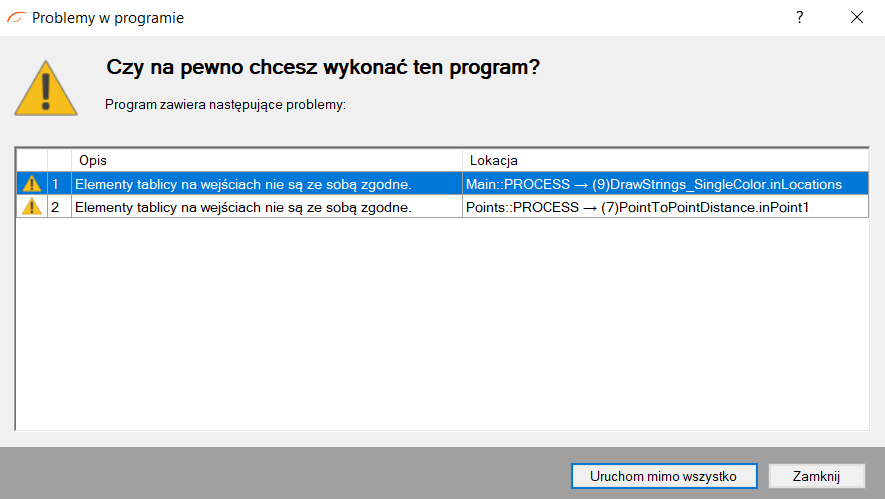
\includegraphics[height = 0.175 \linewidth]{img2}%
	}%
	\hfill%
	\subfloat[Uproszczenie]{%
		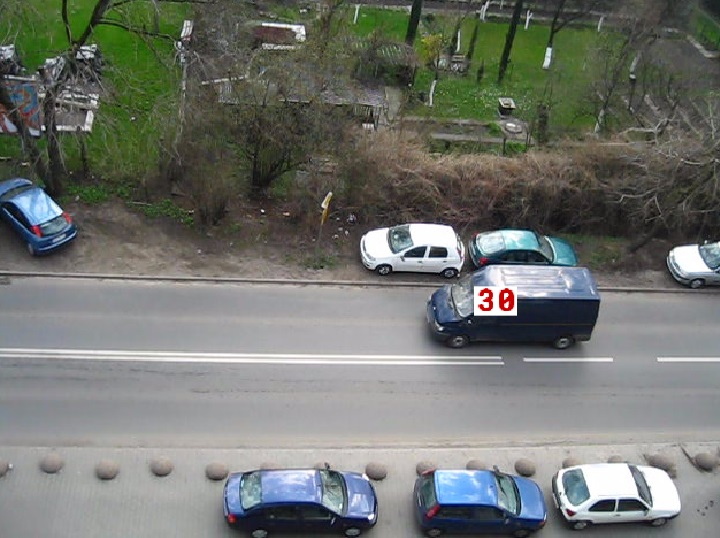
\includegraphics[height = 0.175 \linewidth]{img4}%
	}%
	
	\caption{Zbrojenie fundamentu}
\end{figure}

Fundament jest prostokątem o wymiarach $a$ x $b$ [m], a oczka siatki to prostokąty o wymiarach $c$ x $d$ [m]. Zatem, cała siatka składa się z:
\begin{itemize}[ ]
\item $\frac{a}{c} + 1$ prętów poziomych,
\item $\frac{b}{d} + 1$ prętów pionowych,
\end{itemize}

By zrozumieć problem dalej, zwróćmy naszą uwagę na jeden pręt z całej siatki.
\begin{figure}[h!]
	\centering
	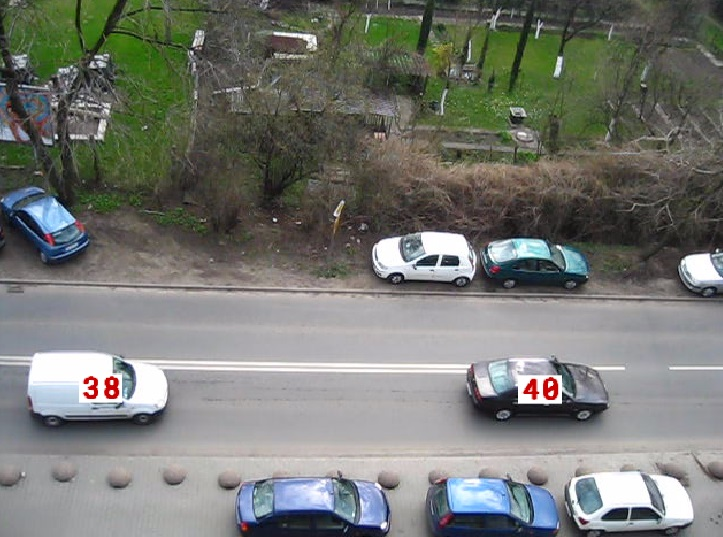
\includegraphics[width = 0.45\linewidth]{img3}
	\caption{Siatka z zaznaczonym jednym prętem}
\end{figure}

\paragraph{Uwaga}
Musimy rozgraniczyć dwa pojęcia: pręty \emph{zakupione} oraz pręty \emph{zbrojeniowe}. Oczywiście, w zadaniu chodzi o to, że pręty z obu tych grup są ze sobą powiązane, ale powiązanie to zostanie wytłumaczone później. Na tym etapie:
\begin{itemize}[--]
\item p. zakupiony -- pręt o długości $e$ metrów, składający się z $p_{1Y_1}$ podprętów.
\begin{equation*}
\mathbf{p}_i = \left[ p_{i1} \ p_{i2} \ \cdots \ p_{1Y_i} \right]
\end{equation*}

\item p. zbrojeniowy -- jeden z prętów siatki prętowej, czyli główny bohater następnego punktu. Jak zostanie wytłumaczone, on także składa się z pewnej liczby prętów.
\end{itemize}

\newpage

\subsection{Jeden pręt zbrojeniowy}

Jeden pręt \emph{zbrojeniowy} może zostalić zrealizowany na kilka sposobów.
\begin{figure}[h!]
	\centering
	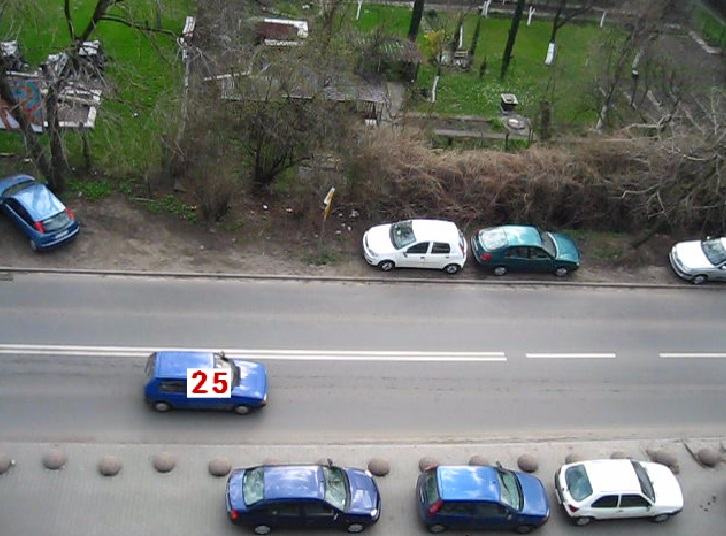
\includegraphics[width = 0.45\linewidth]{img5}
	\caption{Jeden pręt zbrojeniowy -- przykładowe rozwiązania}
\end{figure}

Opis rozwiązań:
\begin{itemize}[--]
\item Pręt nr 1 -- składa się z jednego pręta,
\item Pręt nr 2 -- składa się z dwóch prętów,
\item Pręt nr 3 -- składa się z dwóch prętów o dłuższym wspólnym fragmencie,
\item Pręt nr 4 -- składa się z czterech prętów.
\end{itemize}

Najłatwiej byłoby po prostu położyć pręt o konkretnej długości $a$ i problem z głowy. Takie podejście po pierwsze może być niemożliwe, a po drugie nawet jeśli jest dopuszczalne, to niekoniecznie (raczej nie) będzie optymalne.

Gdy konstruujemy jeden pręt zbrojeniowy z kilku krótszych prętów, należy zastosować zakładkę, czyli obszar na którym będą one się wspólnie nakładały na siebie. Zakładka ma minimalną długość $i$ [m], ale ograniczenia maksymalnego już nie ma. Pręty nr 2 i 3 to pokazują.

Czym więcej prętów tym więcej zakładek, co pokazuje przykład nr 4.

\subsection{Zapis matematyczny}

Zakładając, że $a$ = 8 m, zapiszmy przykład z góry korzystając z wektorów:
\begin{align*}
\mathbf{u}_1 &= \left[ 8 \right] \\
\mathbf{u}_2 &= \left[ 4.2 \ 4.2 \right] \\
\mathbf{u}_3 &= \left[ 4.5 \ 4.5 \right] \\
\mathbf{u}_4 &= \left[ 2.5 \ 3 \ 1.5 \ 2.25 \right]
\end{align*}

Każdy z prętów składa się z pewnej liczby krótszych prętów -- podobnie jak przy zakupie. Jednak, tym razem nie ma ograniczenia równościowego na elementy wektorów $\mathbf{u}$, jest za to ograniczenie nierównościowe -- czym więcej prętów tym więcej zakładek, czyli tym dłuższa musi być suma elementów wektorów. Nie musi ona jednak być jakaś konkretna, jest tylko ograniczenie nierównościowe.
\begin{align*}
\sum_{j = 1}^{1} u_{1j} & = 8 \\
\sum_{j = 1}^{2} u_{2j} & = 8.4 \\
\sum_{j = 1}^{2} u_{3j} & = 9 \\
\sum_{j = 1}^{4} u_{4j} & = 9.25
\end{align*}

Spójrzmy ponownie na pręt nr 4 z rysunku przykładowego:
\begin{figure}[h!]
	\centering
	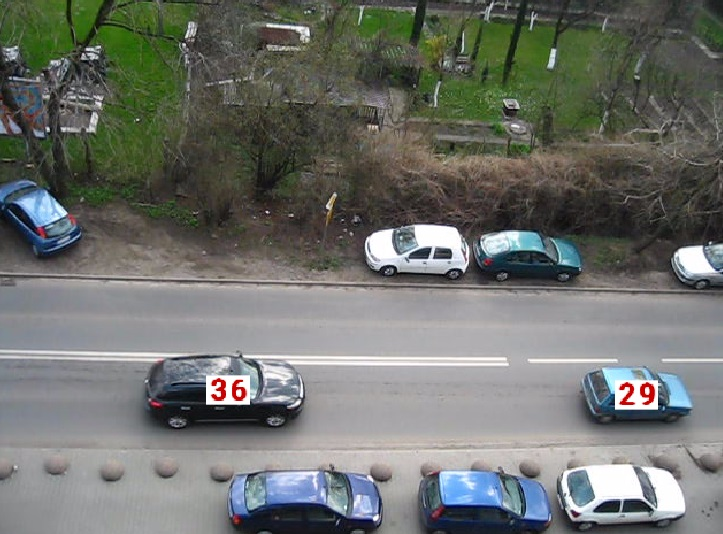
\includegraphics[width = 0.6\linewidth]{img6}
	\caption{Rozsunięcie prętów}
\end{figure}

Pręt 4a to pręt nr 4 z poprzedniego rysunku, a pręt 4b to to samo rozwiązanie, ale pręty nie nachodzą na siebie -- zostały przesunięte. Teraz widać, że czym więcej prętów tym ich wspólna długość jest większa.

\subsubsection*{Równanie stanu}
Proponujemy opis korzystając z równania stanu:
\begin{equation*}
x_{n+1} = x_n + u_n
\end{equation*}

Sterowania $u_n$ opisują długość pręta $n$-tego, a stan $x_n$ to suma długości $n$ położonych prętów.
\begin{equation*}
x_0 = 0 \qquad x_N \ge a + (N - 1) \cdot 2 \cdot i
\end{equation*}

Startujemy oczywiście z zera ($x_0 = 0$), ale na stan końcowy nałożone jest ograniczenie nierównościowe. W zależności od tego ile ($N$) prętów zostało użytych, tym dłuższa musi być ich wspólna długość -- wystarczająco duża, by pokryć minimalne zakładki $i$. Sam stan końcowy $x_N$ oraz liczba użytych prętów $N$ jest na tym etapie niewiadoma, i musi zostać zaproponowana przez algorytm rozwiązujący zadanie.
\begin{equation*}
i \le u_i \le f
\end{equation*}

Ograniczenia nałożone na sterowanie wynikają z tego, że pręty muszą być co najmniej dłuższe niż zakładka $i$, ale krótsze niż $f$, czyli ograniczenie nałożone na transport.

\subsection{Opis całej siatki}
Każdy jeden pręt zbrojeniowy jest opisywany przy pomocy równania stanu. Siatka składa się jednak z wielu prętów i tym samym każdy pręt otrzymuje swoje własne równanie stanu i wektory sterowań/stanów.
\begin{figure}[h!]
	\centering
	\includegraphics[width = 0.75\linewidth]{img7}
	\caption{Siatka z wektorami stanu}
\end{figure}

Cała siatka składa się z $M$ prętów zbrojeniowych. Jest $R$ prętów poziomych i $M$ - $R$ prętów pionowych. Dokładne wartości wynikają z parametrów $a$, $b$, $c$, $d$, a proponowane przez nas wzory zostały zapisane na początku rozdziału.


Wektory sterowań dla każdego prętu siatki:
\begin{align*}
\mathbf{u}_1 &= \left[ u_{10} \ u_{11} \ \cdots \ u_{1K_1} \right] \\
\mathbf{u}_2 &= \left[ u_{20} \ u_{21} \ \cdots \ u_{2K_2} \right] \\
& \vdots \\
\mathbf{u}_i &= \left[ u_{i0} \ u_{i1} \ \cdots \ u_{iK_i} \right] \\
& \vdots \\
\mathbf{u}_M &= \left[ u_{M0} \ u_{M1} \ \cdots \ u_{MK_M} \right] \\
\end{align*}

Wektorami stanu $\mathbf{x}_i$, są o jeden element dłuższe.

Każdy pręt zbrojeniowy siatki składa się z $K_i$ + 1 prętów. Dokładna wartość $K_i$ zależy od rozwiązania problemu optymalizacji.

Wzory/ograniczenia na stan/sterowanie zostały przedstawione wcześniej, ale trzeba wziąć pod uwagę raz jeszcze ograniczenie nierównościowe na stan końcowy:
\begin{equation*}
x_{iN_i} \ge
	\begin{cases}
	a + (N_i - 1) \cdot 2 \cdot i \qquad \text{dla} \ i \in \{1, 2, \ldots, R\} \\
	b + (N_i - 1) \cdot 2 \cdot i \qquad \text{dla} \ i \in \{R+1, R+2, \ldots, M\}
	\end{cases}
\end{equation*}

Długość ,,startowa'' ($a$, $b$) zależy od tego czy analizujemy pręt poziomy czy pionowy.

\newpage
}{}

\ifthenelse{\equal{\value{num}}{0} \OR \equal{\value{num}}{4}}{
\section{Powiązanie}
W poprzednich rozdziałach zaproponowaliśmy opis zakupionych prętów oraz siatki prętów. Opisy te zawierają dużo różnych macierzy i jeszcze więcej innych zmiennych pomocniczych służących głównie do opisów wymiarów wektorów. Teraz należy połączyć jedną część z drugą.

Chodzi o to, że musimy połączyć pręty z wektorów $\mathbf{p}_i$ (pręty zakupione) z prętami z wektorów $\mathbf{u}_i$ (pręty zbrojeniowe). Zasada jest następująca:
\begin{equation*}
\forall_{p_{ij}} \ \exists!_{u_{mk}} \ p_{ij} = u_{mk}
\qquad \land \qquad
\forall_{u_{mk}} \ \exists!_{p_{ij}} \ u_{mk} = p_{ij}
\end{equation*}

W sposób prosty i elegancki cała myśl mogła zostać zapisana przy pomocy języka matematyki. Jeszcze raz, bardziej po ludzku:
\begin{center}
Dla każdego pręta $p_{ij}$ (zakupionego) istnieje \\ dokładnie jeden pręt $u_{mk}$ (zbrojeniowy) i vice versa.
\end{center}

To samo, w sposób graficzno-matematyczny (zakładając macierzowy, a nie wektorowy, sposób zapisu prętów):
\begin{figure}[h!]
	\centering
	\includegraphics[width = 0.75 \linewidth]{img8}
	\caption{Powiązanie pomiędzy elementami}
\end{figure}

\subsection*{Co stanowi duży problem?}
Każdy zakupiony pręt, wraz z jego podprętami, może powędrować w zupełne inne miejsca siatki, co dobrze widać na rysunku powyżej. Z tego powodu, jest nam ciężko rozwiązać problem i otrzymać optymalne parametry zakupu.

\newpage
}{}

\ifthenelse{\equal{\value{num}}{0} \OR \equal{\value{num}}{5}}{
\section{Końcowy zapis problemu}
Postarajmy się zgrupować wszystko to do czego doszliśmy.

\subsubsection*{Zakupione pręty}

To ile prętów kupiliśmy, i z jakich części się one składają zapisujemy w postaci wektorów $\mathbf{p}_i$:
\begin{align*}
\mathbf{p}_1 &= \left[ p_{11} \ p_{12} \ \cdots \ p_{1Y_1} \right] \\
\mathbf{p}_2 &= \left[ p_{21} \ p_{22} \ \cdots \ p_{2Y_2} \right] \\
& \vdots \\
\mathbf{p}_i &= \left[ p_{i1} \ p_{i2} \ \cdots \ p_{iY_i} \right] \\
& \vdots \\
\mathbf{p}_U &= \left[ p_{U1} \ p_{U2} \ \cdots \ p_{UY_U} \right] \\
\end{align*}

Czyli kupiliśmy $U$ prętów, a każdy pręt składa się z $Y_i$ podprętów.

Ograniczenia na zakupione pręty są dwa:
\begin{itemize}[--]
\item dla każdego pręta, suma jego podprętów musi dawać $e$ metrów (jedynie taką możliwość daje nam sklep):
\begin{equation*}
\forall_{i \in \{1, 2, \ldots, U\}} \ \sum_{j = 1}^{Y_j} p_{ij} = e
\end{equation*}
\item każdy podpręt musi my niedłuższy niż $f$ (ograniczenie transportowe):
\begin{equation*}
\forall_{i \in \{1, 2, \ldots, U\}} \
\forall_{j \in \{1, 2, \ldots, Y_i\}} \
p_{ij} \le f
\end{equation*}
\end{itemize}

\subsubsection*{Funkcja celu}
Chcemy zapłacić jak najmniej, a płacimy $J$:
\begin{equation*}
\text{min} \ \leftarrow \ J = U \cdot 6 \cdot e + \sum_{i = 1}^{U} (1 - Y_i) \cdot g
\end{equation*}

gdzie:
\begin{itemize}[ ]
\item $U$ -- ilość kupionych prętów,
\item $e$ -- cena za 1 metr pręta,
\item $Y_i$ -- ilość podprętów pręta $i$-tego,
\item $g$ -- cena za jedno cięcie.
\end{itemize}

\subsubsection*{Siatka prętów}

Cała siatka prętów składa się z $M$ prętów zbrojeniowych, w tym: $R$ prętów poziomych, $M - R$ prętów pionowych. Każdy pręt zbrojeniowy jest opisany poprzez równanie stanu:
\begin{equation*}
x_{in+1} = x_{in} + u_{in},
\end{equation*}

i ograniczenia:
\begin{equation*}
x_{i0} = 0 \qquad
x_{iN_i} \ge
	\begin{cases}
	a + (N_i - 1) \cdot 2 \cdot i \qquad \text{dla} \ i \in \{1, 2, \ldots, R\} \\
	b + (N_i - 1) \cdot 2 \cdot i \qquad \text{dla} \ i \in \{R+1, R+2, \ldots, M\}
	\end{cases}
\end{equation*}

Ograniczenie na sterowania to:
\begin{equation*}
i \le u_{in} \le f,
\end{equation*}

czyli pręty muszą być dłuższe niż minimalna zakładka ($i$), ale krótsze niż ograniczenie transportowe ($f$).

\subsubsection*{Powiązanie}
Dla każdego pręta $p_{ij}$ istnieje dokładnie jeden pręt $u_{mk}$:
\begin{equation*}
\forall_{p_{ij}} \ \exists!_{u_{mk}} \ p_{ij} = u_{mk}
\qquad \land \qquad
\forall_{u_{mk}} \ \exists!_{p_{ij}} \ u_{mk} = p_{ij}
\end{equation*}

\newpage
}{}

\ifthenelse{\equal{\value{num}}{0} \OR \equal{\value{num}}{6}}{
\section{Podsumowanie}
Nasza praca kończy się na tym etapie. Zaproponowany przez nas opis zadania powoduje, że znalezienie rozwiązania optymalnego jest dla nas zbyt trudne. Być może problem da się opisać w inny bardziej elegancki sposób, jednak tego już nam się nie udało zrobić. Najbardziej problematyczne w naszym zapisie jest to, że pręty zakupione i zbrojeniowe opisujemy na dwa różne sposoby (wektory $\mathbf{p}$, $\mathbf{u}$), a ich elementy są ze sobą jasno powiązane, ale ,,porozstrzelane'' -- połączenia mogą znajdować się w zupełnie różnych miejscach.

Być może, zdefiniowane przez nas zadanie optymalizacji da się łatwo rozwiązać, ale tego także nie udało nam się wykonać. Najważniejszy dla nas był opis zadania i liczymy na to, że to wykonaliśmy poprawnie.


}{}

\end{document}